\chapter{Path Planning} \label{ch:pp}
The goal of each of the planners introduced is to assist in the discovery of a field's features with an adjustable trade off between speed and confidence of prediction. The user of such a system could choose to scan more area if fuel is not of high concern. Likewise, if the field is very large, or several fields need to be scanned in a limited amount of time, a quicker scan with a lower degree of prediction certainty can be performed.

\section{Field Uncertainty Model} \label{sec:fielduncert}
The hypothesis that intentionally suppressing prediction variance yields a higher quality field prediction is used as the basis of the path planners introduced. The root mean square (RMS) error of any estimator is composed of two parts: a bias and variance of the estimate about the bias. The RMS error is reduced by reducing the variance of estimates. A Best Linear Unbiased Prediction method, such as the Kriging method, can therefore produce higher quality estimates with lower prediction variances.

A method for calculating the variance of a prediction was defined as a function of the proximity vector and Kriging weights generated for the prediction point in Equation \ref{eq:krigvar}. For points that have been directly measured, the variance is ideally zero (for fields with no drift or dynamics). The uncertainty of the prediction of a point in the target field is the variance of its prediction. The goal of a path planner intending to suppress uncertainty of all predictions in a target field would be to reduce the overall variance of the target field being explored.

Let $\Sigma(\cdot)$ be a criterion for overall predicted field uncertainty. The function can be defined as the average variance calculated from a prediction of all $h\times w$ predictable points on a target field from a set of observations, $S$.

\begin{equation}
	\Sigma(\hat{Z}_{S}) = \frac{1}{hw}\sum_{i = 1}^{hw} \text{var}\{\hat{Z}_{S}(\vect{p}_i)\}
	\label{eq:fielduncert}
\end{equation}

\noindent where $\Sigma(\hat{Z}_{S}) \in \mathbb{R}_{\geq 0}$ and $\text{var}\{\hat{Z}_{S}(\vect{p}_i)\} \in \mathbb{R}_{\geq 0}$ is the variance of the prediction of the $i^{th}$ point, $\vect{p}_i$, when the field is predicted from a set of samples, $S$.

\subsection{Uncertainty Loss Function} \label{sec:lossfunc}
A criterion for overall field uncertainty was introduced in Section \ref{sec:fielduncert}. Given a set of sampled points, $S$ on a field, the overall field uncertainty is the mean variance of all points on the field, $\Sigma(\hat{Z}_{S})$. For an additional set of samples, $T$, taken on the field, a new field uncertainty, $\Sigma(\hat{Z}_{S \cup T})$, is the field uncertainty criterion of the fields prediction from the union of the sample sets $S$ and $T$. The difference in overall field uncertainty, $L(T)$, will be defined as the uncertainty lost by taking the additional samples in the set $T$ on the field.

\begin{equation}
	L(T) = \Sigma(\hat{Z}_{S}) - \Sigma(\hat{Z}_{S \cup T})
	\label{eq:lossfunc}
\end{equation}

% The optimal path, $O$, subject to a limited scanning time constraint, is the path that simultaneously maximizes $L(S,O)$, and minimizes the length of of the path taken (using the assumption of a constant linear velocity from Section \ref{sec:vehicledynamics}).

% \begin{equation}
% 	O = \argmax_T\ \beta L(T) - (1-\beta)l(S + T)
% \end{equation}

% \noindent where $\beta \in [0,1]$ is a real number which puts more emphasis on exploration time over prediction quality. It is important to note that as more samples are taken, the overall field prediction variances change. It would be in the benefit of a path planner to batch process a set of points after meeting a predetermined waypoint, or after a threshold number of samples. 

% Given an endpoint in a single trajectory, in the limit, recalculating $O$ at every sample would optimally shape the trajectory of the exploration vehicle. With no endpoint selected, the exploration vehicle could be found in a repeating state due to being stuck in a global minimum in the variance field. In an effort to avoid the sticking minimum problem, the path planners introduced will be endpoint oriented (where the endpoint of any trajectory is predetermined), and the goal of each path taken is to make it to the endpoint. Furthermore, a new path will only be calculated as a batch process after sampling a trajectory. This is done in an attempt to reduce computation time as the Kriging predictions and variance calculations become more expensive as more samples are taken.

% \section{Finding Points of Highest Uncertainty} \label{sec:highestvars}
% Points on a target field with high prediction uncertainties should be sampled in order to reduce overall field uncertainty. After sampling an initial set of points, and then running a Kriging prediction on all points on a target, the variance of prediction of all points can be calculated.

% The motivation of the path finders introduced is to minimize the average uncertainty of a target field by sampling the points representing the highest prediction variances on the field. A set of points where the highest uncertainties lie are found on the field using a simple search.

% Let $S_k$ be a singleton set containing the point of highest variance on the $k^{th}$ iteration of the target field prediction variances, represented as the set $\text{var}\{\hat{Z}_k\}$, where $\text{var}\{\hat{Z}\} : \mathbb{R}^2 \to \mathbb{R}^+$.

% \begin{equation}
% 	S_{k} = \argmax_{\vect{s}} \ \text{var}\{\hat{Z}_{k}(\vect{s})\}
% 	\label{eq:highestvar}
% \end{equation}

% \noindent The cardinality of the set $S_k$ can be greater than one if there exist multiple instances of the same value of variance in the target field prediction variances. For the sake of simplicity, only the singleton case will be considered.

% Let $\text{var}\{\hat{Z}_{k+1}\}$ be the set of points, not including the point of highest variance found in the $k^{th}$ iteration of the set configuration (Equation \ref{eq:highestvar}), on a target field prediction.

% \begin{equation}
% 	\text{var}\{\hat{Z}_{k+1}(\vect{s})\} = \text{var}\{\hat{Z}_k(\vect{s})\} - S_k \\
% 	\label{eq:nextmaxvarsset}
% \end{equation}

% \noindent Let $S_{v}$ be the set of the $N$ points of highest uncertainty on the target field prediction variances, $\text{var}\{\hat{Z}\}$.

% \begin{equation}
% 	\label{eq:highestvarsunion}
% 	S_{v} = \bigcup_{k = 1}^{N} S_k = \bigcup_{k = 1}^{N} \text{var}\{\hat{Z}_k(\vect{s})\} - \text{var}\{\hat{Z}_{k+1}(\vect{s})\}
% \end{equation}

\section{Path Planning Overview}
Five variance suppressing path planners are introduced in this thesis. Each of five path planners attempts to reduce Kriging prediction variance by steering an exploration vehicle through a target field in a fashion that is predicted to reduce overall field uncertainty. All five of the path planners introduced will need an initial set of samples to make an initial path decision. Each of the five path planners begin by conducting an initial sweep on the main diagonal of the field. They initially stop at a waypoint set to a point close to the middle point on the field. The first point is the point in which the zig-zag method (discussed in Section \ref{sec:zz}) initially stops. The initial set of samples taken from the sweep will then be used to make an initial decision.

\section{Highest Variance Path Planner} \label{sec:nhvpp}
The \textit{Highest Variance} (HV) Path Planner attempts to reduce field prediction uncertainty by setting the exploration vehicle's destination to the point of highest prediction variance on the field. After meeting the point of highest variance, the field prediction and variances are recalculated from the samples the vehicle took on its path to the previously selected destination point. The next destination, or \textit{decision point}, is then set to the new point of highest prediction uncertainty.

Sampling the location of the highest variance is the simplest and most naive approach to path planning using the Kriging method. The highest point of uncertainty on the field is the point, $\vect{p}$, is defined as:

\begin{equation}
\argmax_{\vect{p}} \ \text{var}\{\hat{Z}(\vect{p})\}
\end{equation}

By simply setting the next decision point of the path to $\vect{p}$, the point of highest uncertainty will be sampled at the end of the path. Once the point is met at the end of the path, a new set of samples gathered from the path to the endpoint will be used to recalculate the statistical patterns of the field to higher degree of quality. A Kriging prediction, variances of those predictions are then run on the field. The path planner continues by setting the next decision point to the point of highest uncertainty after recalculating the variances of the field. The planner terminates exploration once a preset maximum scan area limit has been met by the exploration vehicle.

\subsection{Inefficiency in Highest Variance Method}
The HV algorithm does not account for repeating paths, or avoiding the re-sampling of points on the field. The only knowledge used is the variance of the endpoint of a path. Although the ground covered by the algorithm may be sufficient for uncertainty suppression, a path planner that considers the cost of trajectories would likely yield better results.

\section{$N$ Highest Variances Path Planner} \label{sec:nnhv}
The \textit{$N$ Highest Variances} (N-HV) Path Planner sets its decision point to a point from a set of the $N$ points of highest prediction variances. A \textit{leg}, or trajectory between the current position of the exploration vehicle and a potential decision point is calculated for all points in the set. The leg that is predicted to reduce the most overall field uncertainty (Equation \ref{eq:fielduncert}) is set as the next decision point of the vehicle. When the decision point is met, the set of legs to the $N$ highest variances is recalculated. The next decision point is set to the point that yields the leg that is expected to maximize loss in field uncertainty.

Let $K_N$ be the set of the $N \in \mathbb{N}$ points of highest uncertainty on the field. Let $T_i$ be a candidate trajectory connecting the current position of the exploration vehicle to the $i^{th}$ point in the set $K_N$. The endpoint that is ultimately chosen by the $N$ Highest Variance Path Planner is the one that maximizes the loss function, $L(T_i)$. The points along a trajectory, $T_i$, have likely not been sampled, as they represent points of high uncertainty. The loss in uncertainty for taking the path, $T_i$, is therefore not known. An estimate of the loss in overall field uncertainty, $\hat{L}(T_i)$, after taking the path, $T_i$, is calculated by using the previous Kriging predictions of the points along the path. The predictions of those points are used as actual samples taken on the field in a new Kriging prediction variance calculation of the field.

\section{Monte Carlo Path Planner} \label{sec:mcpp}
The Monte Carlo Path Planner (MCPP) calculates a set of legs to the $N$ highest points of variance on the field, similarly to the $N$-HV planner, except that for each leg, a separate set of $M_{mc}$ random trajectories are calculated around the leg. The exploration vehicle trajectory, or set of waypoints to a decision point, that is selected, is the random trajectory that maximizes loss in field uncertainty. The samples taken along the last trajectory selected are stored and used to recompute field variances when the final point in the trajectory (decision point) is met. New possible trajectories are then recalculated, and the planner repeats until a predefined maximum exploration distance has been met by the vehicle. This method compares a total of $N M_{mc}$ noisy trajectories per decision point met. By introducing noise into each of the trajectories found in the $N$-HV path planner, a more optimal path may be found.

Let $K_N$ be the set of the $N$ points of highest prediction variances on the field. Let $T_i$ be a candidate trajectory from the current position of the exploration vehicle to the $i^{th}$ endpoint in the candidate endpoint set, $K_N$. Each point in the candidate trajectory is a waypoint the exploration vehicle will visit on its way to the last point in the sequence. The trajectory is a set of states representing the field position, $(x,y)$, and the vehicle heading angle, $theta$. The $k^{th}$ vector in the state candidate trajectory set, $T_i$, denoted as $T_{i}(k)$, will be the state the exploration vehicle will take on at that position on the field, i.e.

\begin{equation}
T_{i}(k) = \begin{bmatrix} x_i(k) \\ y_i(k) \\ \theta_i(k) \end{bmatrix}
\end{equation}

Let $\alpha \in \mathbb{R}$ be the step size of the vehicle from one point to the next within the trajectory, $T_i$. Let $\vect{w}_i \in \mathbb{R}^2$ be a vector of two zero-mean Wiener processes with a tunable process standard deviation which is less than the step size, $\alpha$. Furthermore, the step size of the vehicle, $\alpha$, can not be a value less than the distance the exploration vehicle can travel in one time-step, $\Delta T$, given a constant vehicle velocity of $V$.

\begin{equation}
\text{var}\{\vect{w}_i\} = \begin{bmatrix} \text{var}\{w_{i_x}\} \\ \text{var}\{w_{i_y}\} \end{bmatrix}
\end{equation}

\begin{equation}
\text{var}\{w_{i_x}\} < \alpha^2
\end{equation}

\begin{equation}
\text{var}\{w_{i_y}\} < \alpha^2
\end{equation}

\begin{equation}
\alpha \geq V \Delta T
\end{equation}

The corresponding Monte Carlo path, or sequence of waypoints the exploration vehicle will make on its way to the candidate endpoint, $\vect{p}_i = [p_x\ p_y]^T$.

\begin{equation}
\label{eq:mcpp}
T_{i}(k) = \begin{cases}
	\begin{bmatrix}
		x_0 \\
		y_0\\
		\text{atan2}(p_y - y_0, p_x - x_0)
	\end{bmatrix} & : k = 1 \\

	\begin{bmatrix}
		\alpha \cos \theta_i(k) \\
		\alpha \sin \theta_i(k) \\
		\text{atan2}(p_y - y_i(k), p_x - x_i(k))
	\end{bmatrix} + \begin{bmatrix} 
		\vect{w}_i(k) \\
		0
	\end{bmatrix} & : 1 < k < \Big\lceil \frac{\|\vect{p} - \vect{s}\|_2}{\alpha} \Big\rceil \\


	\begin{bmatrix} p_x \\ p_y \\ 0\end{bmatrix} & : k = \Big\lceil \frac{\|\vect{p} - \vect{s}\|_2}{\alpha} \Big\rceil \\

\end{cases}
\end{equation}

\noindent where the initial point in the candidate trajectory is set to the current position, $\vect{s}=[x_0\ y_0]^T$ from the state vector of the exploration vehicle. Due to the uncertainty in length of the random trajectory generated, the number of waypoints in the candidate trajectory $T_i$ is fixed, such that $k \in [1, \Big\lceil \frac{\|\vect{p}- \vect{s}\|_2}{\alpha} \Big\rceil]$ (the number of points in the trajectory for a step size, $\alpha$, given zero variance noise added to the process). The last point in the candidate trajectory set is set to the corresponding endpoint from the set $K_N$.

\begin{figure}[hbt!]
	\centering
	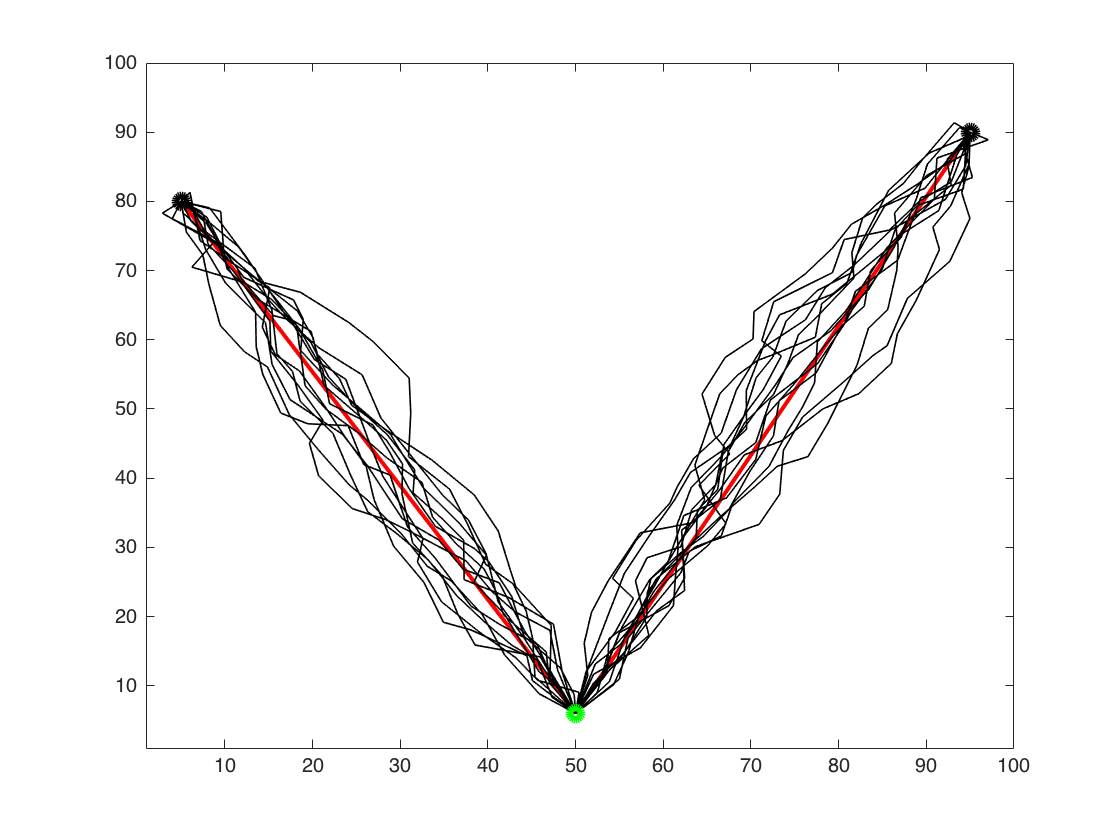
\includegraphics[width=0.8\linewidth]{figures/brownian_motion_mc.png}
	\ssp
	\caption{Monte Carlo paths (black) surrounding deterministic $N$-HV paths (red). The starting point, ($\vect{s} = [50 \ 6]^T$), is indicated in green. The set $K_N$ contains $N=2$ endpoints ($K_N = [ 5 \ 80 ]^T, [ 95 \ 90]^T$). $M_{mc}=15$ random walks are generated for each endpoint. $\alpha=5$. The variance of the Wiener process states are $\frac{1}{2} \alpha$.}
\end{figure}

As introduced in the $N$-HV path planner, a candidate trajectory is generated for each of the candidate endpoints in the set, $K_N$. The candidate trajectory that maximizes the loss function, $L(T)$, is the path that is ultimately selected as the next vehicle trajectory. In an effort to find a more optimal trajectory, more than one random walk can be generated for each endpoint in the set $K_N$. The variable $M_{mc} \in \mathbb{N}$ will denote the number of random walks taken per endpoint in the set $K_N$.

% \begin{algorithm}[h!]
% \caption{Monte Carlo Path Planning (MCPP) with The Kriging Method}\label{alg:mcpp}
% \begin{algorithmic}[1]
% \Procedure{Kriging\_MCPP}{$Z$}
% 	\BState \emph{Conduct Initial Sweep}:
% 	\State SetWaypoint($[h\ w]^T$)
% 	\BState \emph{Krig The Field}:
% 	\State $\hat{Z}, \text{var}\{\hat{Z}\}$ = KrigingPredictField($Z$, $S$)

% 	\BState \textbf{while} $F > 0$ \textbf{and} $\Sigma_{\text{var}} > 0$:
% 	\State $P = []$
% 	\State $\Sigma_{\text{min}} = \infty$ \\

% 	\BState \ \ \ \ \emph{Find the highest field variances}:
% 	\State \ \ \ \ \textbf{for}\ $k = 1 \text{:} N$
% 	\State \ \ \ \  \ \ \ \ $S_{v}(k) = \argmax_{\vect{s}} \ \text{var}\{\hat{Z}_{k}(\vect{s})\}$
% 	\State \ \ \ \ \ \ \ \ $\text{var}\{\hat{Z}_{k+1}(\vect{s})\} = \text{var}\{\hat{Z}_{k}(\vect{s})\} - S_{v}(k)$\\

% 	\BState \ \ \ \  \emph{Calculate trajectories to all points found}:
% 	\State \ \ \ \  $\forall s_k \in S_{v}(k)$:
% 	\State \ \ \ \  \ \ \ \ $s_d = s_k$
% 	\State \ \ \ \  \ \ \ \ $f = \Big\lceil \frac{\|\vect{s}_c - \vect{s}_d\|_2}{\alpha} \Big\rceil$
% 	\State \ \ \ \  \ \ \ \ $T(1) = \begin{bmatrix} s_{c_x} \\ s_{c_y} \\ \text{arctan2}(s_{d_y} - s_{c_y}, s_{d_x} - s_{c_x}) \end{bmatrix}$
% 	\State \ \ \ \  \ \ \ \ $\forall i \in (1, f - 1)$:
% 	\State \ \ \ \  \ \ \ \  \ \ \ \ $T(i+1) = T(i) + \begin{bmatrix} \alpha \cos \theta(i) \\ \alpha \sin \theta(i) \\ \text{atan2}(s_{d_y} - T(i)_y, s_{d_x} - T(i)_x) \end{bmatrix} + \begin{bmatrix} \vect{w}(i) \\ 0 \end{bmatrix}$
% 	\State \ \ \ \  \ \ \ \ $T(f) = \begin{bmatrix} s_{d_x} \\ s_{d_y} \\ \theta_{f-1} \end{bmatrix}$\\

% 	\BState \ \ \ \  \ \ \ \  \emph{Calculate estimated field confidence for trajectory computed}:
% 	\State \ \ \ \  \ \ \ \  $\forall i \in [1, f]$:
% 	\State \ \ \ \  \ \ \ \  \ \ \ \ $\text{samples}(\hat{S}_T)$ += $\hat{Z}(T(i))$
% 	\State \ \ \ \  \ \ \ \  \ \ \ \ $\text{locations}(\hat{S}_T)$ += $T(i)$
% 	\State \ \ \ \  \ \ \ \  \ \ \ \ $\hat{Z}_T, \text{var}\{\hat{Z}\}_T$ = KrigingPredictField($Z$, $\hat{S}_T$)
% 	\State \ \ \ \  \ \ \ \  \ \ \ \ $\Sigma_{\text{var}}(T) = \text{avg}(\text{var}\{\hat{Z}\}_T)$\\

% 	\State \ \ \ \  \ \ \ \  \ \ \ \ \textbf{if} $\Sigma_{\text{var}}(T) < \Sigma_{\text{min}}$ \textbf{and} \text{length($T$)} $< F$:
% 	\State \ \ \ \  \ \ \ \  \ \ \ \ \ \ \ \ $\Sigma_{\text{min}} = \Sigma_{\text{var}}(T)$
% 	\State \ \ \ \  \ \ \ \  \ \ \ \ \ \ \ \ $P = T$\\

% 	\BState \ \ \ \  \emph{Navigate through the chosen path}:
% 	\State \ \ \ \  $\forall p \in P$:
% 	\State \ \ \ \  \ \ \ \ SetWaypoint($p$) 
% \EndProcedure
% \end{algorithmic}
% \end{algorithm}

% In Algorithm \ref{alg:mcpp}, the function \texttt{SetWaypoint()} is an abstracted function which steers the vehicle in the direction of the waypoint specified, and blocks the code instruction until the waypoint has been met. The function \texttt{length(}$T$\texttt{)} finds the arc length of the path by connecting all points in the trajectory, $T$. For a deterministically calculated trajectory, $T$, the arc length is $\alpha |T|$.

\section{The Gradient Ascent Path Planner}
The Gradient Ascent (GA) Path Planner reduces field prediction variance by maximizing the movement in the local variance field's gradient at every move. At every decision point, a circle, with radius $r \in \mathbb{R}_{\geq 0}$, is generated around the exploration vehicle. In order to approximate the field variance gradient surrounding the exploration vehicle, a small step size value for $r$ is chosen. In this thesis, $r=3$ vesicles is used. The point on the circle surrounding the exploration vehicle with the highest Kriging prediction variance is set as the next decision point.

\section{The Range Gradient Ascent Path Planner}
The Range Gradient Ascent (RGA) Path Planner is similar to the Gradient Ascent path planner, but it sets the radius of the candidate circle surrounding the exploration vehicle to the value of the range, $a$, on the field's variogram, i.e. ($r = a$). The points within the range circle are points that are considered spatially autocorrelated, and therefore predictable to a high degree of confidence. By navigating the exploration vehicle to a point on the edge of spatial autocorrelation, the vehicle is motivated to move to points of higher prediction variance as the planner continues to run.

\section{Other Planners}
The five planners introduced will be compared to two planners discussed in the Section \ref{sec:prev_works} on Previous Works. The first method, the zig-zag (ZZ) method, directs the exploration vehicle through a predetermined path which spirals through the entirety of the field. The second method, the Greedy Next-Best-View (NBV) \cite{fentanes:soilkrig}, attempts to reduce Kriging variance by redirecting an exploration vehicle to the point of highest prediction variance after each sample taken.

\subsection{Zig-Zag Method} \label{sec:zz}
A common approach to exploration and patrolling problems is the use of a zig-zag pattern. The methods introduced will be compared to a zig-zagging approach demonstrated in Nikhil Nigam, et al. \textit{Control and Design of Multiple Unmanned Air Vehicles for a Persistent Surveillance Task} (Part II.C.3, Figure 6, \cite{nigam:zigzag}). The method will run a Kriging prediction and variance calculation on the samples taken using the zig-zag explorer, even though a prediction is not specified in the original work. This is to generate measurable and comparable metrics against the path planners introduced.

The zig-zag exploration method will stop the field exploration process when the exploration vehicle traverses a predefined area to scan, $A_{scan}$. If the maximum scan area of a field is $w \times h$, and the percent of the field to scan is $p\%$, then the method will stop exploring when the area $A_{scan} = \frac{p}{100}wh$ of the field has been sampled. The spacing between each spiral bound, $r$, will be pre-calculated in an effort to allow the zig-zag method to cover as much of the field as possible.

\begin{equation}
	\label{eq:zigzagrad}
    r = \frac{100}{p}
\end{equation}

The zig-zag method starts at the first point on the field (upper-left corner), and moves to the waypoint coordinate ($\Large\lceil\frac{w}{2} - r \Large\rceil, \Large\lceil \frac{h}{2} - r \Large\rceil$). Every planner will set the initial waypoint of the exploration vehicle to this point on the field. This is done so the initial set of samples of each of the planners is identical.

\subsection{Greedy Next-Best-View ($20 \times 20$)}
The Greedy NBV method, demonstrated in \cite{fentanes:soilkrig}, triggers the selection of a new waypoint after every new sample is taken by the exploration vehicle. The point that is chosen is the point on the field with the highest Kriging prediction variance at the time of point selection. After the next sample is taken on the way to the point of highest variance, the planner recomputes the field's variogram model, Kriging prediction, and field variance to recalculate the next decision point. The Greedy NBV planner will initiate by conducting an initial sweep on the main diagonal of the field and stop at the middle point of the field. This is done in order to collect a set of samples to make an initial decision.

\section{Discussion on the Planners Introduced} \label{sec:discuss}
The Monte Carlo path planner takes into account a set of noisy trajectories, and compares their estimated return on investment similarly to the $N$-HV method. Given enough trajectories, as $N$ gets larger for $N$-HV and MCPP and $M_{mc}$ gets larger for MCPP, the planners could find a path that will reduce overall field uncertainty in a more brute-force way over the HV, GA, and RGA methods introduced. The disadvantages of MCPP and $N$-HV lie in the fact that the cost of each next move taken is not considered directly because an entire trajectory is considered, in its entirety, at once. A more optimal approach to this planner would be to take into consideration the cost of each waypoint selected on the trajectory, and amend only the best waypoints found along the way. Furthermore, the MCPP approach is more computationally expensive (for $N > 1$, $M_{mc} > 1$) when compared to HV and $N$-HV because of the need to re-predict the field for each candidate trajectory calculated. The GA method becomes more computationally expensive as more samples are taken on the field, as this makes it more difficult to recompute the variogram model and Kriging predictions for the field at each step of the path. The HV, GA, and RGA planners are the simplest to compute because they only require one run of the Kriging field predictions and variance calculations, followed by a simple search for the highest field variances from a specified set of points.

The Greedy Next-Best-View planner, though similar to the GA and RGA planners introduced, does not purposefully attempt to directly sample the point of highest prediction variance from a set of candidate points. Both the GA and RGA planners arrive at a point of high variance from a set of candidate points, and sample it, where as the Greedy NBV will only move in the direction of the point of highest variance. As the field sizes get larger, the point of highest variance could be relatively distant from the point that is actually explored using Greedy NBV. The Greedy NBV method is therefore not expected to do well for larger fields. This is because the exploration vehicle can run into the problem where it will stick in a low variance valley. Once trapped in the valley, the vehicle will repeatedly move between two previously explored points until the end condition is met. The method will only be compared to the introduced methods in this thesis using course as presented in \cite{fentanes:soilkrig}.

A preplanned method, like the zig-zag method, does not intentionally attempt to suppress overall field prediction uncertainty, and because of this, may not predict the states of interest of the field to a high enough degree of accuracy when compared to the direct variance suppression methods. The zig-zag method does however attempt to sample an even distribution of path across the target field, allowing the method to estimate the field states to a high degree of accuracy.